%!TeX spellcheck = en-US

%\chapter{Evaluation Methodology for WGI and Computational Text Categorization}
\chapter{Evaluation framework for open-set WGI}

\label{chap:eval_methods}

%----------------------------------------------------------------------------------------

% Define some commands to keep the formatting separated from the content
\newcommand{\keyword}[1]{\textbf{#1}}
\newcommand{\tabhead}[1]{\textbf{#1}}
\newcommand{\code}[1]{\texttt{#1}}
\newcommand{\file}[1]{\texttt{\bfseries#1}}
\newcommand{\option}[1]{\texttt{\itshape#1}}

%----------------------------------------------------------------------------------------

\section{Introduction}\label{chap:eval_methods:sec:intro}

This chapter is describing the evaluation metrics required for the open-set WGI task. Particularly it is shown with simple examples the effect of the a measurement methods to the evaluation results and the misleading conclusions on can have when the wrong measurement method is adopted. Moreover some evaluation measures are presented specialized for the open-set framework where recently have been discover and adopted for several domains inside and outside the \textit{text mining} domain.

The standard evaluation approach is to use a previously well tested evaluation methodology and measures. However, the closed-set measures is later shown that they are not proper for the open-set framework in their standard form. 

To reason it in few words the problem is that these measures are based on the \textit{Confusion Matrix} which can capture only two condition per variable. However, in the case of open-set framework there is one say "global" condition where all the variables of the table drops. This condition is occurring when the \textit{rejection condition} of the open-set algorithm is triggered. That is when an open-set algorithm responds "I don't know" for an arbitrary sample. 

As explained in chapter \ref{chap:openset} there are some efforts to crate open-set algorithms than could model the \textit{unknown} or \textit{unstructured noise} samples. In this case it could be possible the out-of-the-box closed-set evaluation methods be sufficient,however, in most ML algorithms where a rejection criterion is considered this is nearly impossible as it will be presented later.

\section{Closed-set vs Open-set Measures}\label{chap:eval_methods:sec:measures} 

In this section it is presented how the text mining evaluation measures are affected by the type of the by the type of the task's approach scenario. That is, whether i
t is an open-set of closed-set classification framework.

Starting with the \textit{Confusion matrix} where the basic closed-set evaluation measures are based it is shown the difference in measure of the Precision and Macro-Precision difference (also for Recall) in the open-set framework. Moreover, it is shown how these measures are affected by he openness score which is the score for evaluating the difficulty level of an open-set problem.

Finally, the \textit{Open Space Risk} is presented which is the measure helping an open-set algorithm to regulate the potentially error in the presence of \textit{noise} in the testing or/and \textit{outages} in the training phase.


\subsection{Confusion Matrix and $F$ Score}\label{chap:eval_methods:sec:prf_micro}

In Machine Learning (and Statistical) Classification, a \textit{Confusion Matrix} is a table that depicts the performance of an algorithm. It is a special case of a \textit{Contingency Table}, with two dimensions, actual and predicted classes. Thus, in the a binary case such as in the table \ref{chap:eval_methods:tbl:bin_confusion}, there are for cases occurring. True Positive (TP), True Negative (TN), False Positive (FP), False Negative (FN).

In the case of binary classification the samples under the class distribution A are desired, i.e. positive, and all the other samples outside the distribution are considered negative, classified in say class B. Then TP and TN are the counts of samples predicted correctly under the a class A (positive) or class B (negative). Therefore, the FP and FN are the samples a binary algorithm misleaded and predicted the wrong class. 

\begin{table}[H]
	\center
	\caption{Confusion matric of binary classification}\label{chap:eval_methods:tbl:bin_confusion}
	\begin{tabular}{c c c c c}
		& & \multicolumn{2}{c}{Actual} & \\
		\cline{3-4}
		\multirow{3}{*}{\rotatebox[origin=r]{90}{Predicted}} & & \multicolumn{1}{|c}{A} & \multicolumn{1}{c|}{B} & \\
		\cline{2-4}
		& \multicolumn{1}{|c}{A} & \multicolumn{1}{|c}{\textbf{50}} & \multicolumn{1}{c|}{30} & 80 \\
		& \multicolumn{1}{|c}{B} & \multicolumn{1}{|c}{25} & \multicolumn{1}{c|}{\textbf{35}} & 60 \\
		\cline{2-4}
		&  & 70 & 70 & \textbf{85}\\
	\end{tabular}
\end{table}

In order to measure the performance a binary classification algorithm the \tetxit{Accuracy} is a common measure which is actually the ration of all the correct prediction overall the predictions (which is equivalent to the number of the samples of the whole data set). Formally, it is shown in the equation \ref{chap:eval_methods:eq:accuracy} and for the example of the table \ref{chap:eval_methods:tbl:bin_confusion} its value is $A = 85/140 = 0.607$

\begin{equation}\label{chap:eval_methods:eq:accuracy}
A = \frac {TP + TN} {TP +  TN + FP + FN}
\end{equation}

However, one can get a better insight when it is measured the algorithms ability distinguishing the samples which they are under the distribution it has been trained for. Moreover, to be measured its ability of recognizing the samples of this distribution. The former is called \textit{Precision} and the second it is called \textit{Recall} and their formal expressions are in equation \ref{chap:eval_methods:eq:precision} and \ref{chap:eval_methods:eq:recall} respectively. 

\begin{equation}\label{chap:eval_methods:eq:precision}
	P = \frac {TP} {TP + FP}
\end{equation}

\begin{equation}\label{chap:eval_methods:eq:recall}
	R = \frac {TP} {TP + FN}
\end{equation}

\textit{Precision} is also known as \textit{Positive Predictive Value (PPV)}. \textit{Recall} is also known as \textit{Sensitivity, Hit Rate and True Positive Rate (TPR)}. Again based on table \ref{chap:eval_methods:tbl:bin_confusion} the precision is the ration its first cell value and the sum of its first row (prediction) which is equal to $p = 50 / 80 = 0.625$. Similarly, recall is equal to the ration of first cell value over the first column, i.e. $r = 50 / 70 = 0.714$

So far one-class closed-set classification was considered where the class A was the positive outcome and the Class B the negative. In the multi-class closed-set classification scenario, an algorithm is trained for both A and B class distribution. Thus, the positive and negative samples are now counted from both classes.

In the same table \ref{chap:eval_methods:tbl:bin_confusion} the \textit{precision} and \textit{recall} is now calculated by the ration of the diagonal sums of 2 diagonals. That is $p = 85 / (85 + 55) = 0.607$ and $r = 85 / (85 + 55) = 0.607$. 

If one would like to consider the performance on class A separately to the performance on class B then the respective calculations are for precision and recall. The ration of the A correct predictions over the whole positive prediction of row A and similarly for B. Thus, $p_{A} = 0.625$ and $p_{B} = 35 / 60 = 0.583$. Moreover, the recall are $r_{A} = 0.714$ and $r_{B} = 35 / 70 = 0.500$.

\subsection{Macro-Precision and Macro-Recall}\label{chap:eval_methods:sec:prf_macro}

The calculation where the positive and negative predictions of both classes are calculated together are called micro-Precision and micro-Recall. In the case where per class calculation of the precision and recall are averaged these scores are called macro-Precision and macro-Recall. 

The macro-P and macro-R for table \ref{chap:eval_methods:tbl:bin_confusion}, are $p_{macro} = 0.604$ and $r_{macro} = 0.607$. There is a slight difference only in micro and macro precision. However, the problem is significantly amplified when the multi-class classification is becoming open-set and also with more classes.

The table \ref{chap:eval_methods:tbl:bin_confusion} has $140$ total samples which is equal either the the row-sums or the column-sums are summed up. In the case of open-set classification some of the samples are remaining as non-classification or as \textit{unknown} where there is no class trained for them. 

In table \ref{chap:eval_methods:tbl:multi_confusion} there are still 140 sample distributed in a seven (7) classes and also with 42 of them remaining as unclassified. Given these cases, the respective per class, macro and micro recall for this confusion matrix are calculated and shown in table \ref{chap:eval_methods:tbl:bin_macro_vs_micro}.

\begin{table}[H]
	\center
	\caption{Confusion metric of binary classification}\label{chap:eval_methods:tbl:multi_confusion}
	\begin{tabular}{c c c c c c c c c c c}
		& & \multicolumn{7}{c}{Classified of Actual} & \\
		\cline{3-10}
		\multirow{9}{*}{\rotatebox[origin=c]{90}{Predicted}} & & \multicolumn{1}{|c}{\emptyset} & \multicolumn{1}{c}{A} & \multicolumn{1}{c}{B} & \multicolumn{1}{c}{C} & \multicolumn{1}{c}{D} & \multicolumn{1}{c}{E}  & \multicolumn{1}{c}{F} & \multicolumn{1}{c|}{G} & \\
		\cline{2-10}
		& \multicolumn{1}{|c}{\emptyset} & \multicolumn{1}{|c}{0} & \multicolumn{1}{c}{\textit{6}} & \multicolumn{1}{c}{\textit{8}} & \multicolumn{1}{c}{\textit{9}} & \multicolumn{1}{c}{\textit{8}} & \multicolumn{1}{c}{\textit{0}} & \multicolumn{1}{c}{\textit{7}} & \multicolumn{1}{c|}{\textit{4}} & 15 \\
		& \multicolumn{1}{|c}{A} & \multicolumn{1}{|c}{0} & \multicolumn{1}{c}{\textbf{13}} & \multicolumn{1}{c}{1} & \multicolumn{1}{c}{1} & \multicolumn{1}{c}{0} & \multicolumn{1}{c}{0} & \multicolumn{1}{c}{0} & \multicolumn{1}{c|}{0} & 15 \\
		& \multicolumn{1}{|c}{B} & \multicolumn{1}{|c}{0} & \multicolumn{1}{c}{1} & \multicolumn{1}{c}{\textbf{10}} & \multicolumn{1}{c}{1} & \multicolumn{1}{c}{0} & \multicolumn{1}{c}{0} & \multicolumn{1}{c}{1} & \multicolumn{1}{c|}{3} & 16 \\
		& \multicolumn{1}{|c}{C} & \multicolumn{1}{|c}{0} & \multicolumn{1}{c}{0} & \multicolumn{1}{c}{0} & \multicolumn{1}{c}{\textbf{1}} & \multicolumn{1}{c}{0} & \multicolumn{1}{c}{0} & \multicolumn{1}{c}{0} & \multicolumn{1}{c|}{3} & 4 \\
		& \multicolumn{1}{|c}{D} & \multicolumn{1}{|c}{0} & \multicolumn{1}{c}{0} & \multicolumn{1}{c}{0} & \multicolumn{1}{c}{1} & \multicolumn{1}{c}{\textbf{8}} & \multicolumn{1}{c}{0} & \multicolumn{1}{c}{0} & \multicolumn{1}{c|}{1} & 10 \\
		& \multicolumn{1}{|c}{E} & \multicolumn{1}{|c}{0} & \multicolumn{1}{c}{0} & \multicolumn{1}{c}{0} & \multicolumn{1}{c}{1} & \multicolumn{1}{c}{2} & \multicolumn{1}{c}{\textbf{20}} & \multicolumn{1}{c}{1} & \multicolumn{1}{c|}{1} & 25 \\
		& \multicolumn{1}{|c}{F} & \multicolumn{1}{|c}{0} & \multicolumn{1}{c}{0} & \multicolumn{1}{c}{0} & \multicolumn{1}{c}{1} & \multicolumn{1}{c}{2} & \multicolumn{1}{c}{0} & \multicolumn{1}{c}{\textbf{10}} & \multicolumn{1}{c|}{0} & 13 \\
		& \multicolumn{1}{|c}{G} & \multicolumn{1}{|c}{0} & \multicolumn{1}{c}{0} & \multicolumn{1}{c}{1} & \multicolumn{1}{c}{5} & \multicolumn{1}{c}{0} & \multicolumn{1}{c}{0} & \multicolumn{1}{c}{1} & \multicolumn{1}{c|}{\textbf{8}} & 15 \\
		\cline{2-10}
		& & 0 & 14 & 12 & 11 & 12 & 20 & 13 & 16 & \textbf{70}\\
		\cline{3-10}
		& & \textit{0} & \textit{20} & \textit{20} & \textit{20} & \textit{20} & \textit{20} & \textit{20} & \textit{20} & 140\\
	\end{tabular}
\end{table}


\begin{table}[H]
	\center
	\caption{Macro and Micro calculation for the Confusion matrix (Table \ref{chap:eval_methods:tbl:bin_confusion}) of binary classification}\label{chap:eval_methods:tbl:bin_macro_vs_micro}
	\begin{tabular}{l l l}
		\cline{2-3}
		& \multicolumn{1}{|c}{Precision} & \multicolumn{1}{c|}{Recall}\\
		\cline{1-3}
		\multicolumn{1}{|c}{A} & \multicolumn{1}{|c}{0.866} & \multicolumn{1}{c|}{0.650}\\
		\multicolumn{1}{|c}{B} & \multicolumn{1}{|c}{0.625} & \multicolumn{1}{c|}{0.500}\\
		\multicolumn{1}{|c}{C} & \multicolumn{1}{|c}{0.250} & \multicolumn{1}{c|}{0.050}\\
		\multicolumn{1}{|c}{D} & \multicolumn{1}{|c}{0.800} & \multicolumn{1}{c|}{0.400}\\
		\multicolumn{1}{|c}{E} & \multicolumn{1}{|c}{0.800} & \multicolumn{1}{c|}{1.000}\\
		\multicolumn{1}{|c}{F} & \multicolumn{1}{|c}{0.769} & \multicolumn{1}{c|}{0.500}\\
		\multicolumn{1}{|c}{G} & \multicolumn{1}{|c}{0.533} & \multicolumn{1}{c|}{0.400}\\
		\cline{1-3}
		\multicolumn{1}{|c}{Macro} & \multicolumn{1}{|c}{0.663} & \multicolumn{1}{c|}{0.500}\\
		\multicolumn{1}{|c}{Micro} & \multicolumn{1}{|c}{0.714} & \multicolumn{1}{c|}{0.500}\\
		\cline{1-3}
	\end{tabular}
\end{table}


Clearly the is a significant difference in the macro-P compare to the micro-P and for this case, micro and macro recalls are have both $0.500$ score. It should be noted that due to the 42 samples of the 140 that haven't been classified at all there is bias over precision score when its micro score is calculated. Moreover, there is problem in calculation of the recall based in the equation form \ref{chap:eval_methods:eq:recall} because in the closed set classification the denominator is equal to the total number pf samples that we know they are under the distribution of the class we are evaluating for. 

The recall calculation issue is cased because of the open-set framework and the sample are renaming out of the classification processing because of the rejection criterion of an open-set algorithm. In order to calculate the recall we are following the theoretical definition of the this score which is formally expressed in equation \ref{chap:eval_methods:eq:recall_theory}.

\begin{equation}\label{chap:eval_methods:eq:recall_theory}
	R = \frac {\text{The sum of correctly classified samples}} {\text{The total number of distribution's testing samples}}
\end{equation}

Thus in the case of \textit{micro-R} is the denominator is equal to the total number of all samples of the data-set. In the \textit{macro-R} case, is the number of the class-samples for every class separately and then the average score recall score of all classes.

In the table \ref{chap:eval_methods:tbl:multi_confusion} the micro recall show that only the $50\%$ of the total samples have been correctly classified and the $98/140 = 70\%$ of the total samples have been classified while the rest has been remained as \textit{unknown}. The macro recall is also $0.5$ based on the separated evaluation for every different class.

However, the precision is much more accurate in the case of macro compare to the micro because the micro precision is bias for the algorithms positive performance since the rejected samples (characterized as unknown) are not calculate in the precision performance or their are not causing any kind of penalty to the precision score. In addition the proper calculation of recall (micro and macro) as explained above will not differ in the extend of regulating the F-score.

The F-Score is the \textit{Harmonic Mean} of two other scores, i.e. the difference between the to score is creating a kind of penalty to the final value. The general calculation function of F-Score is the shown equation \ref{chap:eval_methods:eq:f_score}

\begin{equation}\label{chap:eval_methods:eq:recall}
	F_{\beta} = (1 + \beta^{2}) \frac {P R} {\beta^{2} P + R}
\end{equation}

\noindent
where $\beta$ in $F_{\beta}$ regulates the weighting bias towards the Precision or Recall score. Usually the $F_{1}$, i.e. with $\beta = 1$, is the used for equally weighted precision and recall significance. Calculating the F-scores for macro and micro scores of the table \ref{chap:eval_methods:tbl:bin_macro_vs_micro} we have $F1_{micro} = 0.588$ and $F1_{macro} = 0.559$.

The macro scores are then less biased for the the open-set framework evaluation. Moreover, in the highly imbalanced corpora also the macro scoring is reported to be more realistic and less biased. Due to the above reasoning the macro-P, macro-R, and Macro-F1 will mainly be the evaluation measure is used in this thesis.

In the next chapter the Precision Recall Curves will be presented where it is more vivid the effect of the micro and macro measurement. That is there it is clear the bias over the precision in the algorithm's performance because of the open-set algorithm criterion.


\subsection{PRC and ROC Curves}\label{chap:eval_methods:sec:roc_prc}

The \tetxit{Precision Recall Curves (PRC)} and the \tetxit{Receiver Operating Characteristic} are two standardized methods for evaluating the Information Retrieval algorithms. Usually is an out-of-the-box choice for ranking systems. They also can be used for classification as long as there is available the probability or any certainty score for the classification. Thus, it can be applied in "soft" classification, while in "hard" classification is possible when the decision scores are available. 

The calculation of the PR curves requires the truth-table sequence for the predictions, ranked in descending order based on the \textit{algorithm's certainty scores}. 


\begin{table}[H]
	\center
	\caption{Macro and Micro calculation for the Confusion matrix (Table \ref{chap:eval_methods:tbl:bin_confusion}) of binary classification}\label{chap:eval_methods:tbl:bin_macro_vs_micro}
	\begin{tabular}{|c|c|c|c|}
		\cline{1-4}
		Certainty & Predicted & Expected & Correct\\
		\cline{1-4}
		0.99 & 1 & 1 & 1 \\
		0.99 & 2 & 2 & 1 \\
		0.99 & 4 & 4 & 1 \\
		... & ... & ... & ... \\
		0.79 & 2 & 6 & 0 \\
		0.79 & 4 & 4 & 1 \\
		0.69 & 7 & 6 & 0 \\
		0.69 & 4 & 4 & 1 \\
		... & ... & ... & ... \\
		0.64 & \emptyset & 6 & 0 \\
		0.60 & 2 & 2 & 1 \\
		... & ... & ... & ... \\
		0.60 & \emptyset & 4 & 0 \\
		\cline{1-4}
	\end{tabular}
\end{table}



\begin{figure}[t]
	\begin{center}
    	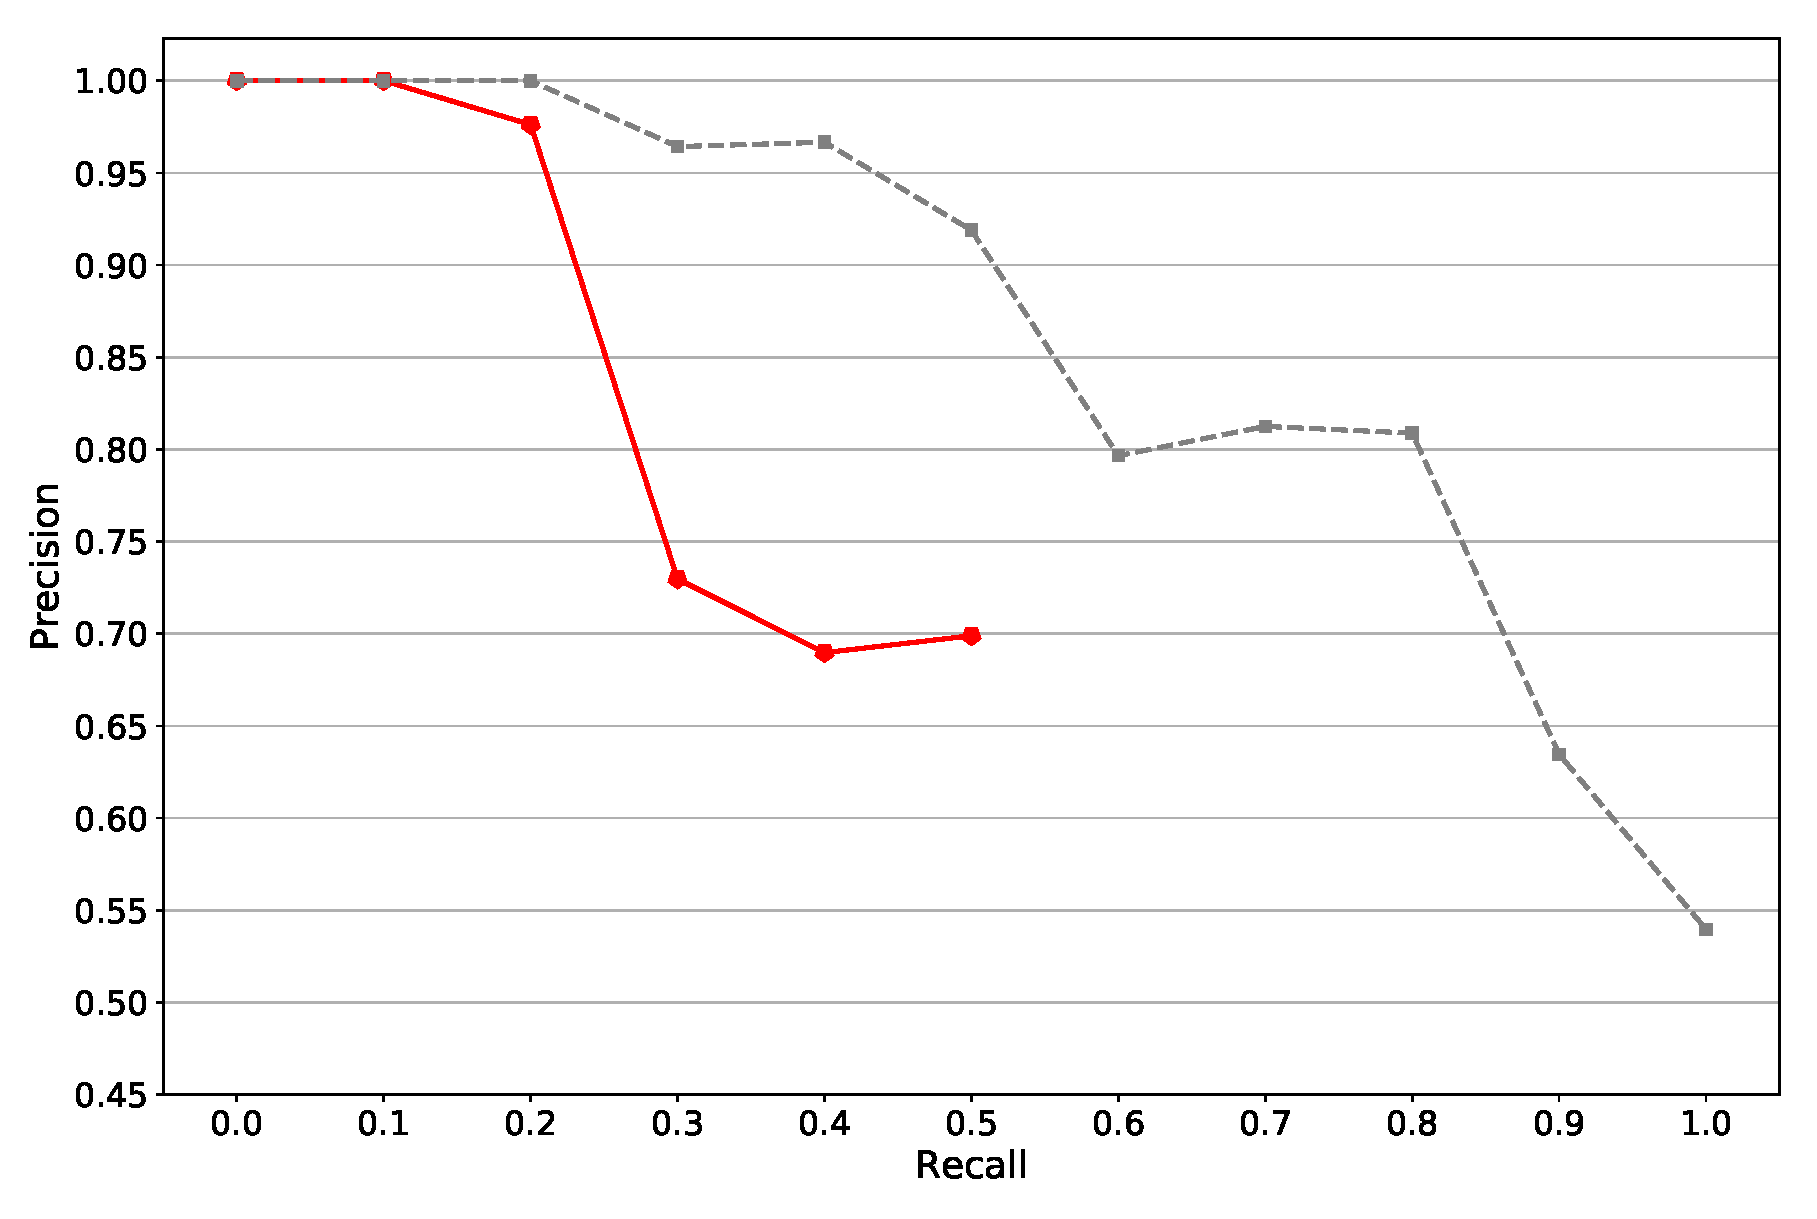
\includegraphics[scale=0.45]{Figures/pr_macro_micro_example.eps}
		\caption{Open-set Macro (Red line) and Micro (grey line) Precision Recall Curves of confusion matrix in table \ref{chap:eval_methods:tbl:multi_confusion}}
		\label{chap:eval_methods:tbl:prc_macro}
	\end{center}
\end{figure}


\section{Area Under the Curve (AUC)}\label{chap:eval_methods:sec:closed_set_classification} 

Precision-Recall curve is a standard method to visualize the performance of classifiers. In this paper, the Precision-Recall curve is calculated in 11-standard recall levels $[0,0.1,...,1.0]$. Precision values are interpolated based on the following formula:

\begin{equation}
	P(r_j)=max_{r_j \leqslant r \leqslant r_{j+1}}(P(r))
\end{equation}

\noindent
where $P(r_j)$ is the precision at $r_j$ standard recall level.


To compensate the potentially unbalanced distribution of web pages over the genres, we are using the macro-averaged precision and recall measures. In more detail, we use the modified version of precision and recall for open-set classification tasks proposed by \parencite{mendesjunior2016}. This modification calculates precision and recall only for the known classes (available in the training phase) while the unknown samples (belonging to classes not available during training) affect false positives and false negatives. To find parameter settings that obtain optimal evaluation performances we use 2 scalar measures, the Area Under the Precision-Recall Curve (AUC)and $F_{1}$. We will show that the appropriate selection of the optimization measure is highly significant in the presence of noise.


\section{Re-defining the Open Space Risk}\label{chap:eval_methods:sec:open_space_risk} 

The open space risk in \parencite{scheirer2013toward} is originally defined as in eq. \ref{chap:eval_methods:eq:the_original_open_space_risk}

\begin{equation}\label{chap:eval_methods:eq:the_original_open_space_risk}
	R_{o}(f) = \frac{\int_{o} f_{y}(x) dx}{\int{S_{o}}  f_{y}(x) dx}

\end{equation}

\noindent
where $R_{o}(.)$ is the open-space risk function and $f_{y}(x)  \in \{0, 1\}$ is the classification function of class $y$, where $1$ is for recognizing its class and $0$ when not. $S_{o}$ is the large hyper-sphere where all the positive training data points and the \textit{positive open space area} $O$. 

The original formulation of the eq. \ref{chap:eval_methods:eq:the_original_open_space_risk} $O$ area cannot be constrained by any means. The only information we are getting is the farther form the training date we go the risk of miss-classification is increasing One method to constrain the problem is by using the center of the positively labeled training data and defining a radios $r_{o}$ where it will reduce the open space area based on the positively labeled empirically observations. Then the $O$ is defined by the equation eq. \ref{chap:eval_methods:eq:openspace_spherical_constrained}

\begin{equation}\label{chap:eval_methods:eq:openspace_spherical_constrained}
	O = S_{o} - B_{r_{y}}(C_{y})
\end{equation}

\noindent
where $B_{r_{y}}(.)$ is the function which defines the area of radius $r_{y}$ of the $C_{y}$ class defined by its training data \parencite{fei2016breaking}.

\section{Openness test}\label{chap:eval_methods:sec:open_space_risk}

In \parencite{scheirer2013toward} work in image processing, the \textit{openness measure} is introduced, as shown in eq. \ref{chap:eval_methods:eq:openness}. The openness measure indicates properties of an open-set classification task by taking into account the number of \textit{training classes}, i.e. the known labels used in the training phase and the number of \textit{testing classes}, i.e., the labels, both known and unknown, used in the testing phase.

\begin{equation}\label{chap:eval_methods:eq:openness}
	openness=1-\sqrt{\frac{ | Training Classes | }{ |Testing Classes | }}
\end{equation}

When openness is $0.0$, it is essentially a closed-set task, that is the training and testing classes are the same or there is no noise. When openness reaches $1.0$ this means that the known classes are far less than the unknown classes, that is the amount of noise is especially high. Therefore, by varying the openness level we can study the performance of WGI models in different conditions.

Note that the openness measure can only be applied to corpora where all available documents have been labeled with genre information. In other words, we have to know the genre labels of the pages that form the noise (i.e. structured noise). Thus, it cannot be applied to SANTINIS corpus where the web pages taken from the SPIRIT collection are unclassified (i.e., unstructured noise). On the other hand, the SANTINIS corpus provides the opportunity to examine WGI performance when all documents not belonging to the known labels are grouped into one single (highly heterogeneous) class.



\section{Domain Transfer Measure}\label{chap:eval_methods:sec:domain_transfer_measure}

A practical methodology for evaluating a classification/identification ML model in a text-categorization task is the \textit{Domain Transfer Evaluation}. The goal of this evaluation methodology is to measure the generalization of the model when training corpus is rather small and to evaluate how the model would perform in an unknown domain for the same task. 

Particularly for the AGI/WGI with this measure we can evaluate a ML algorithm when for example the model has been trained to identify \textit{News} and \textit{Wiki} genres, however, the available corpus would be only from \textit{Technology products Topics}. Then by testing it on {Sports Topics} we could evaluate the model in such a case when very small corpus is available for training. In addition using this methodology we can evaluate the models behavior depending on the \textit{Features} have been selected for the training, e.g. BOW, POS, Term N-grams etc. 

One can measure the performance, say Accuracy, F1-statistic, Precision-Recall Curve,  Receiver Operating Characteristic (ROC) Curve etc, and then compare the two measures pairwise for every domain combination (e.g. $\{Mobile Phones, Football\}$, etc). However, it would be easier to have measure for all possible combinations training/testing of different domain combinations. 

The measure proposed from \parencite{finn2006learning} and shown in equation \ref{eq:gnr_dom_transit_general} in its generalized form. Originally, this measure was designed for Accuracy measure in mind. However, it can be used for any measure say $F_{1}$-statistic in order to fit in open-set framework and not respected to the closed-set also (Να ελέγξω αν το Accuracy μπορεί να χρησιμοποιηθεί για Open-set). 

\begin{equation} \label{chap:eval_methods:eq:office_doc_ensemble}
	T^{C,F} = \frac{1}{N(N-1)} \sum_{A=1}^{N} \sum_{B, \forall B \neq A}^{N} \left(  \frac{M^{C,F}_{A,B}}{M^{C,F}_{A,A}} \right)
	\end{equation}

	\noindent	
where T is the \textit{Transfer Measure Score}, M is the measure of choice (Accuracy, $F_1$, Precision, Recall, etc), F is the \textit{Feature Set}, and C is the \textit{Genre Class}. 
























